\documentclass[11pt]{article}
\usepackage[utf8]{inputenc}
\usepackage{circuitikz}
\usepackage{stmaryrd}
\usepackage{titlesec}
\usepackage{graphicx}
\usepackage{amsmath}
\usepackage{amssymb}
\usepackage[txtcentered=true, height=40pt, width=70pt]{thumbs}
\usepackage{float}
\usepackage{color}
\usepackage[left=2.5cm, top=2.5cm, right=3cm]{geometry}
\usepackage[justification=centering]{caption}
\DeclareGraphicsExtensions{.png}

\newcommand{\fancythumb}[2]{
	\addthumb{#1}{\large\sffamily\textbf{\space\space#1\vspace{5pt}}}{white}{#2}
}

\pagenumbering{arabic}
\titleformat*{\section}{\sffamily\huge\bfseries}
\titleformat*{\subsection}{\sffamily\Large\bfseries}
\titleformat*{\subsubsection}{\sffamily\large\bfseries}

\begin{document}
\section*{Gleichstrommaschine}
\fancythumb{GSM}{teal}

\newpage
\section*{Asynchronmaschine}
\fancythumb{ASM}{red}
\subsection*{Einphasiges Ersatzschaltbild}
\begin{figure}[h]\centering
	\begin{circuitikz}[european, scale=1, font=\large]
	\draw
		(0,3)
		to [short, i=$\underline{I}_1$, o-](1.0,3)
		to [L=$L_{\sigma1}$](3,3)
		to [short](4.0,3)
		to [L=$L_{h1}$, i>_=$\underline{I}_{m1}$, *-*] (4,0)
		(4.0,3.0)
		to [L=$L_{\sigma2}'$](7.0,3.0)
		to [R=$R_{2}' ~ \frac{1}{s}$, i>^=$\underline{I}_1^i$](10.0,3)
		to [R, l_=$R_{2Z}' ~ \frac{1}{s}$] (10.0,0) 
		to [short, -o]	(0,0);

	\draw[->, >=latex] (0,2.8) -- (0,0.2) node [pos=0.5, left] {$\underline U_1$};
	\end{circuitikz}
	\caption*{Man beachte die schlupfabhängigen Widerstände}
\end{figure}

\subsection*{Leistungsbilanz}
\begin{figure}[h]
	\centering
	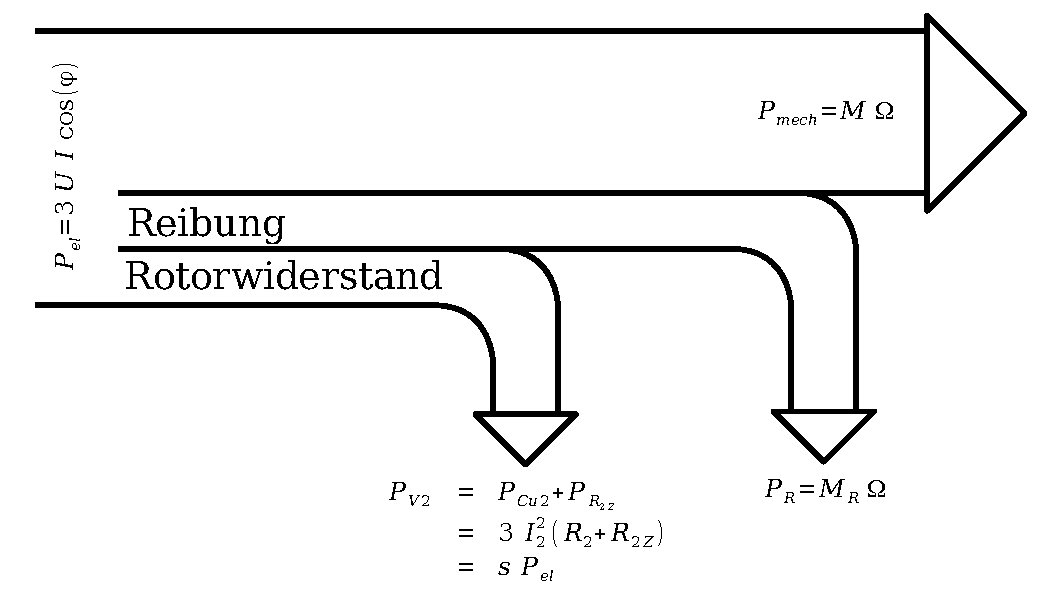
\includegraphics[width=0.7\textwidth]{img/asynchronmaschine_leistungsbilanz.pdf}
	\caption*{Sonstige Verluste vernachlässigt, mit $I_2$…Läuferstrom, häufig gilt $R_{2Z} = 0$}
\end{figure}

\subsection*{Kenngrößen}
\subsection*{Stromortskurve (Heylandkreis)}
\subsection*{Momentenkennlinie}
\subsection*{Formeln}

\newpage
\section*{Synchronmaschine}
\fancythumb{SM}{magenta}

\newpage
\section*{Transformator}
\fancythumb{Trafo}{olive}

\newpage
\section*{Drehstromverbraucher}
\fancythumb{\huge $\Yup ~ \mathrm{/} ~ \triangle$}{darkgray}

\newpage
\section*{Anhang}
\fancythumb{Anhang}{black}
\subsection*{Herleitung Schlupfgerade Asynchronmaschine}
\begin{figure}[h]
	\centering
	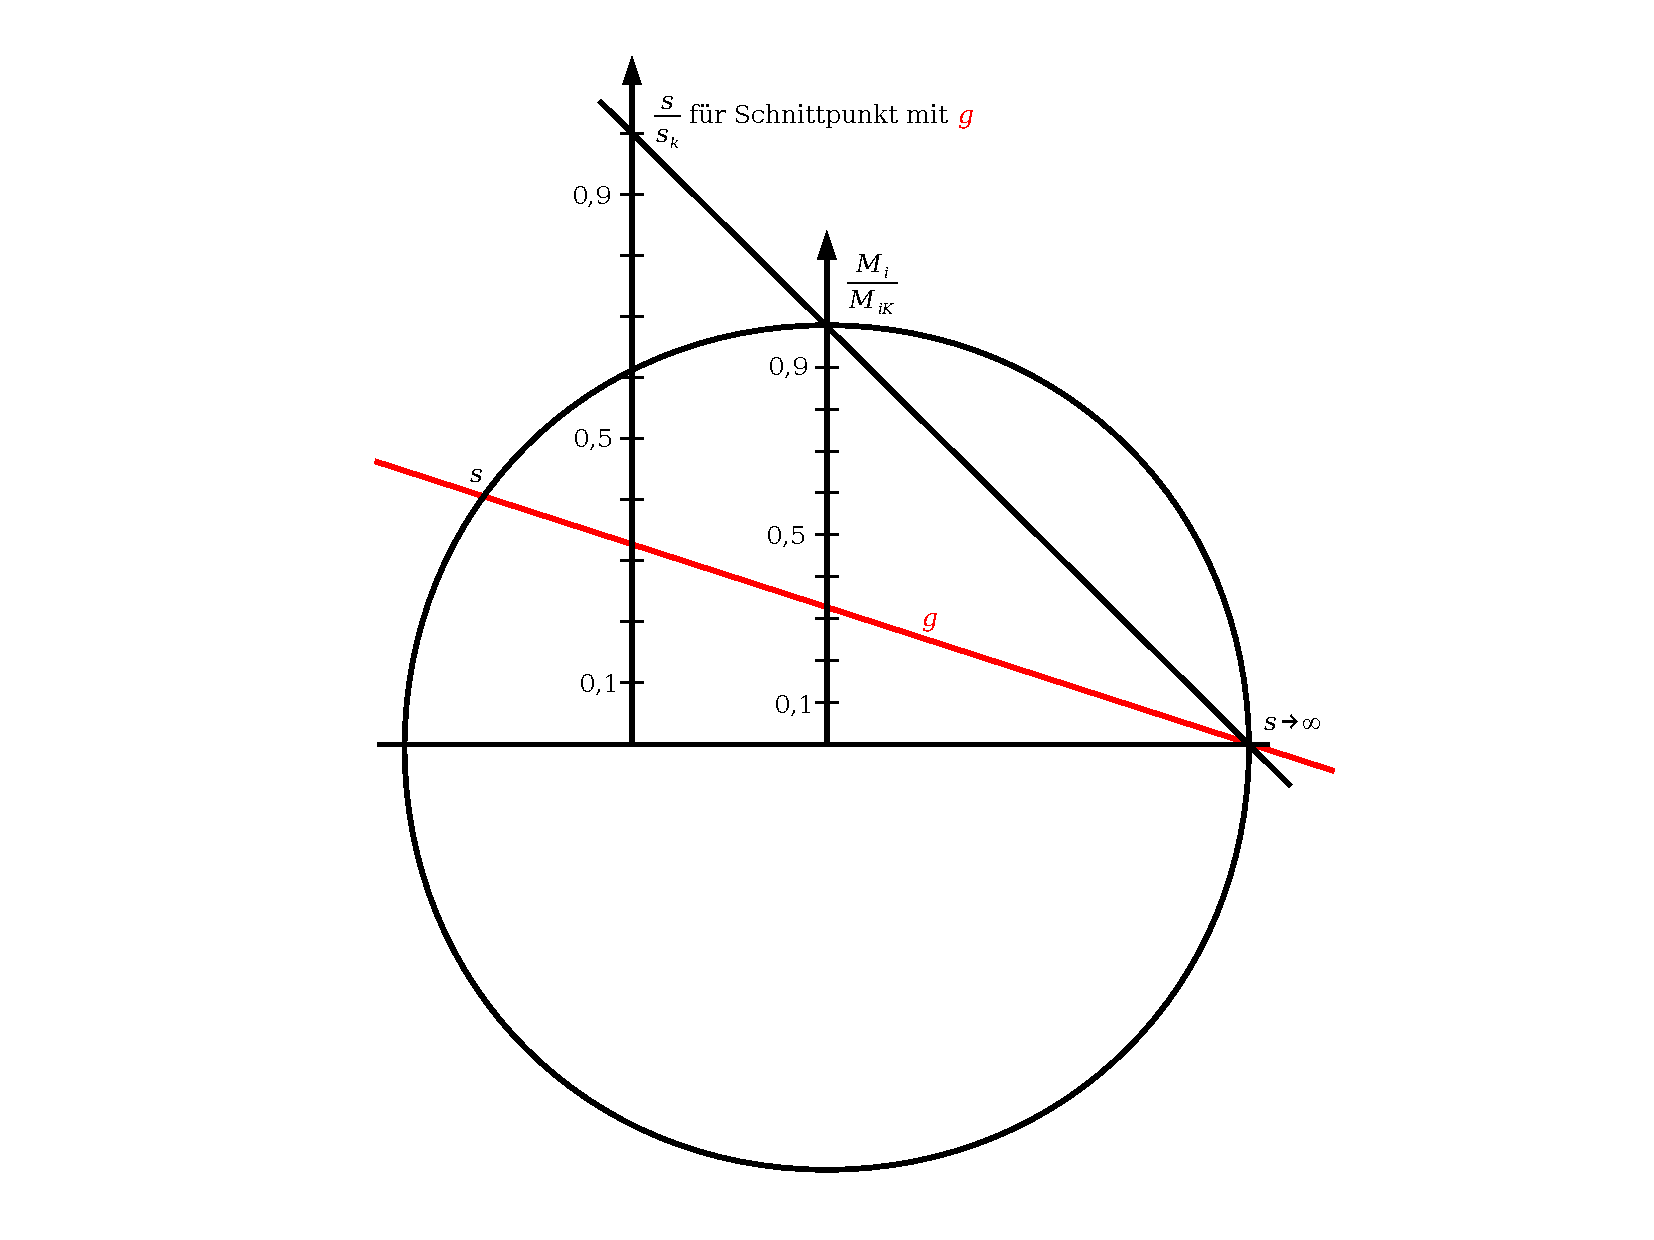
\includegraphics[width=0.8\textwidth]{img/asynchronmaschine_schlupfgerade_verschoben.pdf}
	\caption*{Heylandkreis - Der Schlupf an Stelle $s$ soll bestimmt werden}
\end{figure}

\paragraph{Problem:} Wir möchten den Wert des Schlupfes für einen beliebigen Punkt auf dem Heylandkreis (die Ortskurve des Statorstroms in der komplexen Ebene) bestimmen. Der Schlupf hat allerdings keinen linearen Zusammenhang mit dem Mittelpunktswinkel. Der Kippschlupf sei bekannt.

\paragraph{Behauptung:} Durch Konstruktion einer Skala $s \over s_k$ wie in der obigen Grafik, sodass der Wert $1,0$ der Skala durch die Gerade vom Punkt $s \to \infty$ durch den Punkt des Kippschlupfes ("oben" im Kreis) gegeben ist, lässt sich der Schlupf eines beliebigen Punktes $s$ auf dem Heylandkreis ablesen. Dazu wird eine Gerade $g$ durch den Punkt $s \to \infty$ und $s$ konstruiert. Der Wert $s \over s_k$ kann nun am Schnittpunkt dieser Gerade mit der Skala abgelesen werden.

\paragraph{Beweis: } Zeige die Behauptung erst für den Fall, dass sich die $s \over s_k$-Skala im horizontalen Mittelpunkt des Kreises befindet und verallgemeinere dann. Der Kreis habe den Radius $1$, da der Zusammenhang $\frac{M_i}{M_{iN}} = \frac{I_{1W}}{I_{1WN}}$ gilt (d.h. Normierung des Stroms auf ein Drehmoment ist erlaubt, ohne die Grafik zu verzerren) und da hier auf das Kippdrehmoment $M_{iK}$ normiert wurde. Für diese Herleitung liege der abzulesende Punkt in der linken Halbebene des Kreises.

\begin{figure}[H]
	\centering
	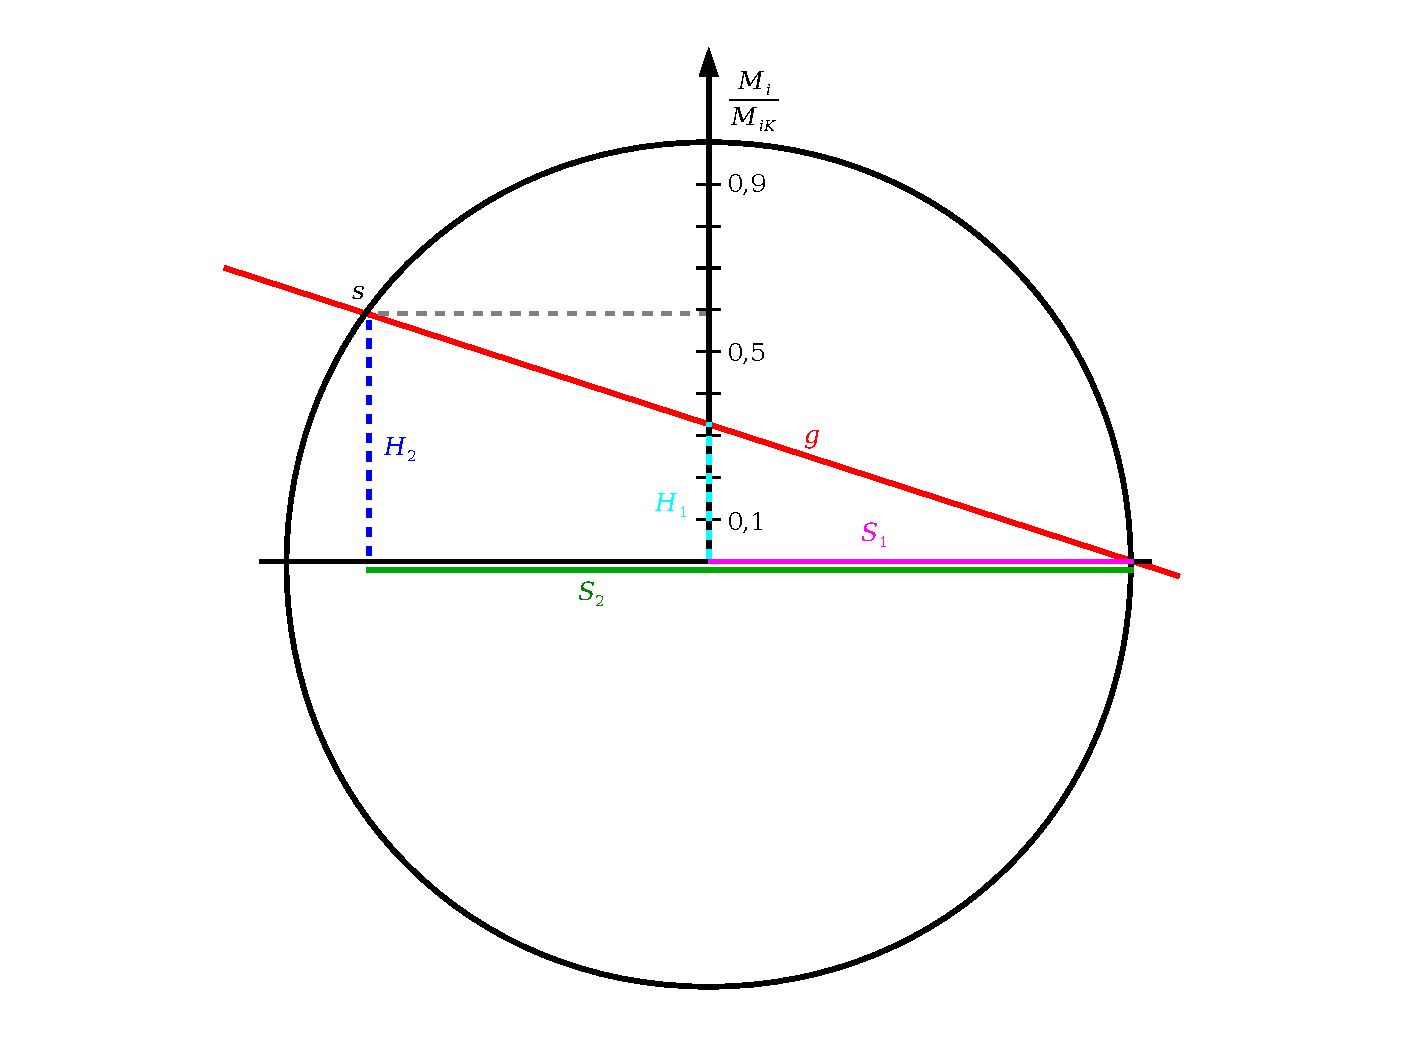
\includegraphics[width=0.8\textwidth]{img/asynchronmaschine_schlupfgerade.pdf}
	\caption*{Schlupfgerade mit Strecken für Strahlensatz}
\end{figure}

Der 2. Strahlensatz lässt mit den Bezeichnungen der Grafik formulieren:
\[
	\frac{H_1}{H_2} = \frac{S_1}{S_2} \implies H_1 = H_2 ~ \frac{S_1}{S_2}
\]

Sei nun das innere Drehmoment des abzulesenden Punktes $M_i$ sowie $M_{ik}$ bekannt. So gilt sofort mit der Normierung auf $M_{iK}$ (Kreisradius 1):
\[
	H_2 = \frac{M_i}{M_{iK}} \quad \mathrm{und} \quad S_1 = 1
\]

$S_2$ kann außerdem einfach aus dem bekannten $H_2$ und dem bekannten Kreisradius 1 berechnet werden:
\[
	H_2^2 + (S_2 - S_1)^2 = 1 \implies S_2 = \sqrt{1 - H_2^2} + S_1 = \sqrt{1 - \left( \frac{M_i}{M_{iK}} \right)^2} + 1
\]

Somit ergibt sich für $H_1$ durch einsetzen in den Strahlensatz:
\[
	H_1 = \frac{\frac{M_i}{M_{iK}}}{\sqrt{1 - \left( \frac{M_i}{M_{iK}} \right)^2} + 1}
\]

Die Behauptung ist nun, dass $H_1 \overset{!}{=} \frac{s}{s_k}$. Dies ist gezeigt, wenn $H_1$ die Kloss'sche Formel erfüllt, d.h.:
\[
	\frac{M_i}{M_{iK}} = \frac{2}{\frac{s}{s_K} + \frac{s_K}{s}} \overset{!}{=} \frac{2}{H_1 + \frac{1}{H_1}}
\]

Berechne $H_1 + \frac{1}{H_1}$:
\begin{align*}
H_1 + \frac{1}{H_1}
		&= \frac{\frac{M_i}{M_{iK}}}{\sqrt{1 - \left( \frac{M_i}{M_{iK}} \right)^2} + 1} + \frac{\sqrt{1 - \left( \frac{M_i}{M_{iK}} \right)^2} + 1}{\frac{M_i}{M_{iK}}} \\
		&= \frac{M_i}{\sqrt{M_{iK}^2 - M_i^2} + M_{iK}} + \frac{\sqrt{M_{iK}^2 - M_i^2} + M_{iK}}{M_i} = \frac{M_i^2 + \left(\sqrt{M_{iK}^2 - M_i^2} + M_{iK}\right)^2}{\left(\sqrt{M_{iK}^2 - M_i^2} + M_{iK}\right)~M_i} \\
		&= \frac{M_i^2 + M_{iK}^2 - M_i^2 + M_{iK}^2 + 2 ~ M_{iK} ~ \sqrt{M_{iK}^2 - M_i^2}}{\left(\sqrt{M_{iK}^2 - M_i^2} + M_{iK}\right)~M_i} \\
		&= \frac{2 ~ M_{iK}^2 + 2 ~ M_{iK} ~ \sqrt{M_{iK}^2 - M_i^2}}{\left(\sqrt{M_{iK}^2 - M_i^2} + M_{iK}\right)~M_i} = \frac{2 \; M_{iK}}{M_i} ~ \frac{M_{iK} + \sqrt{M_{iK}^2 - M_i^2}}{\sqrt{M_{iK}^2 - M_i^2} + M_{iK}} = 2 ~ \frac{M_{iK}}{M_i}
\end{align*}

Einsetzen in die Kloss'sche Formel ergibt:
\[
	\frac{M_i}{M_{iK}} \overset{!}{=} \frac{2}{2 ~ \frac{M_{iK}}{M_i}} \Leftrightarrow 1 = 1
\]

Das heißt, der auf der vertikalen Gerade durch den Kreismittelpunkt abgelesene, normierte Wert ist tatsächlich das gesuchte $s \over s_k$-Verhältnis. Ein Verschieben der Gerade ändert bei entsprechender Anpassung der Skala den abgelesenen Wert nicht ($\rightarrow$ Strahlensatz), somit gilt auch die anfängliche Behauptung. Der Beweis für Punkte auf dem Kreis in anderen Quadranten erfolgt analog. $\square$

\end{document}